\chapter{Conclusioni}
\label{chap:conclusioni}
\section{Consuntivo finale}

L'attività di \textit{stage} ha seguito un piano di lavoro ben definito con obiettivi chiari.
Tutte le attività svolte hanno dato un esito positivo e hanno dato un prodotto più che sufficiente.
Durante il periodo di stage, ci sono stati momenti di difficoltà che hanno rallentato lo sviluppo.
Le principali problematiche incontrate sono state legate alla gestione della \gls{monorepog}\glox e all'implementazione dell'autenticazione nel \gls{backendg}\glox.
Ritengo che questo periodo sia stato molto utile sia per me che per l'azienda, poiché tutto il lavoro svolto ha contribuito a migliorare la gestione di queste problematiche per il futuro.
Ho collaborato attivamente con i membri del \textit{team} Unox e ogni momento di difficoltà è diventato un'opportunità di discussione costruttiva.
L'obiettivo non era solo risolvere i problemi, ma anche comprenderli e prevenire simili situazioni in futuro.
Lo sviluppo delle pagine richieste è stato valutato positivamente dall'azienda.
Nella tabella \ref{tab:requisiti_soddisfatti} sono riepilogati gli obiettivi e i requisiti raggiunti:

\pagebreak
\subsection{Requisiti raggiunti}


\begin{center}
    \rowcolors{1}{}{tableGray}
    \begin{longtable}{|p{2.25cm}|p{5cm}|}
    \hline
    \multicolumn{1}{|c|}{\textbf{Identificatore}} & \multicolumn{1}{c|}{\textbf{Soddisfatto/non}} \\
    \hline 
    \endfirsthead
    \rowcolor{white}
    \multicolumn{2}{c}{{\bfseries \tablename\ \thetable{} -- Continuazione}}\\
    \hline
    \multicolumn{1}{|c|}{\textbf{Identificatore}} & \multicolumn{1}{c|}{\textbf{Soddisfatto/non}} \\
    \hline 
    \endhead
    \hline
    \rowcolor{white}
    \multicolumn{2}{|r|}{{Continua nella prossima pagina...}}\\
    \hline
    \endfoot
    \endlastfoot
    
    RFN-1 & Soddisfatto  \\
    RFN-2 & Soddisfatto  \\
    RFN-2.1 & Soddisfatto  \\
    RFN-2.2 & Soddisfatto  \\
    RFD-2.2.1 & Soddisfatto  \\
    RFN-3 & Soddisfatto  \\
    RFN-3.1 & Soddisfatto  \\
    RFN-4 & Soddisfatto  \\
    RFN-5 & Soddisfatto  \\
    RFN-5.1 & Soddisfatto  \\
    RFN-5.2 & Soddisfatto  \\
    RFN-5.3 & Soddisfatto  \\
    RFN-6 & Soddisfatto  \\
    RFN-6.1 & Soddisfatto  \\
    RFN-7 & Soddisfatto  \\
    RFN-7.1 & Soddisfatto  \\
    RQN-1 & Soddisfatto  \\
    RQN-2 & Soddisfatto  \\
    RVN-1 & Soddisfatto  \\
    RVN-2 & Soddisfatto  \\
    \hline

    \hiderowcolors
    \caption{Tabella dei requisiti soddisfatti.}
    \label{tab:requisiti_soddisfatti}
    \end{longtable}
\end{center}

Come si vede dalla tabella \ref{tab:requisiti_soddisfatti} tutti i requisiti sono stati soddisfatti.
Il piano di lavoro è stato modificato nel momento in cui si è fatta l'analisi dei requisiti.
Fin dall'inizio sono stati delineati requisiti specifici dettagliandoli solo per gli obiettivi realizzabili.

\pagebreak
\subsection{Raggiungimento degli obiettivi}

\begin{center}
    \rowcolors{1}{}{tableGray}
    \begin{longtable}{|p{5cm}|p{2.75cm}|p{4cm}|}
    \hline
    \multicolumn{1}{|c|}{\textbf{Obiettivo}} & \multicolumn{1}{c|}{\textbf{Tipologia}} & \multicolumn{1}{c|}{\textbf{Raggiunto/non}} \\
    \hline 
    \endfirsthead
    \rowcolor{white}
    \multicolumn{3}{c}{{\bfseries \tablename\ \thetable{} -- Continuazione}}\\
    \hline
    \multicolumn{1}{|c|}{\textbf{Obiettivo}} & \multicolumn{1}{c|}{\textbf{Tipologia}} & \multicolumn{1}{c|}{\textbf{Raggiunto/non}} \\
    \hline 
    \endhead
    \hline
    \rowcolor{white}
    \multicolumn{3}{|r|}{{Continua nella prossima pagina...}}\\
    \hline
    \endfoot
    \endlastfoot
    
    Architettura dell'applicazione & Obbligatorio & Raggiunto  \\
    Autenticazione & Obbligatorio & Raggiunto  \\
    Product Page & Obbligatorio & Raggiunto  \\
    Serviced Oven & Obbligatorio & Raggiunto  \\
    Test piattaforme & Obbligatorio & Raggiunto  \\
    RMA & Desiderabile & Non Raggiunto  \\
    Test E2E & Facoltativo & Non Raggiunto  \\
    \hline

    \hiderowcolors
    \caption{Tabella degli obiettivi raggiunti.}
    \label{tab:obiettivi_raggiunti}
    \end{longtable}
\end{center}
Quasi tutti gli obiettivi di sviluppo dello \textit{stage} sono stati raggiunti. Il flusso di lavoro dei \gls{rmag}\glox non è stato avviato in quanto avrebbe richiesto troppo tempo, e si è deciso di dedicare le risorse ad attività con maggiore priorità. L'obiettivo dei test \gls{e2eg}\glox, proposto da me per il progetto, è stato riconosciuto come utile.
Fin dall'inizio, ho ritenuto importante trovare una metodologia pratica per realizzare test \textit{E2E} integrabili nella \gls{cicdg}\glox e che siano multipiattaforma.
Anche in questo caso, si è deciso di concentrare gli sforzi su attività più rilevanti.

Il resto degli obiettivi sono stati raggiunti con successo, permettendo di consegnare un prodotto utilizzabile dall'azienda e conforme alle loro richieste.

\section{Applicazione consegnata}

È stata consegnata l'applicazione \gls{ddcserviceg}\glox funzionante e disponibile in \textit{development} su \textit{iOS}, \textit{Android} e \textit{web}.
Tra le pagine e le funzionalità realizzate, vorrei evidenziare le seguenti:

\begin{figure}[H]
    \centering
    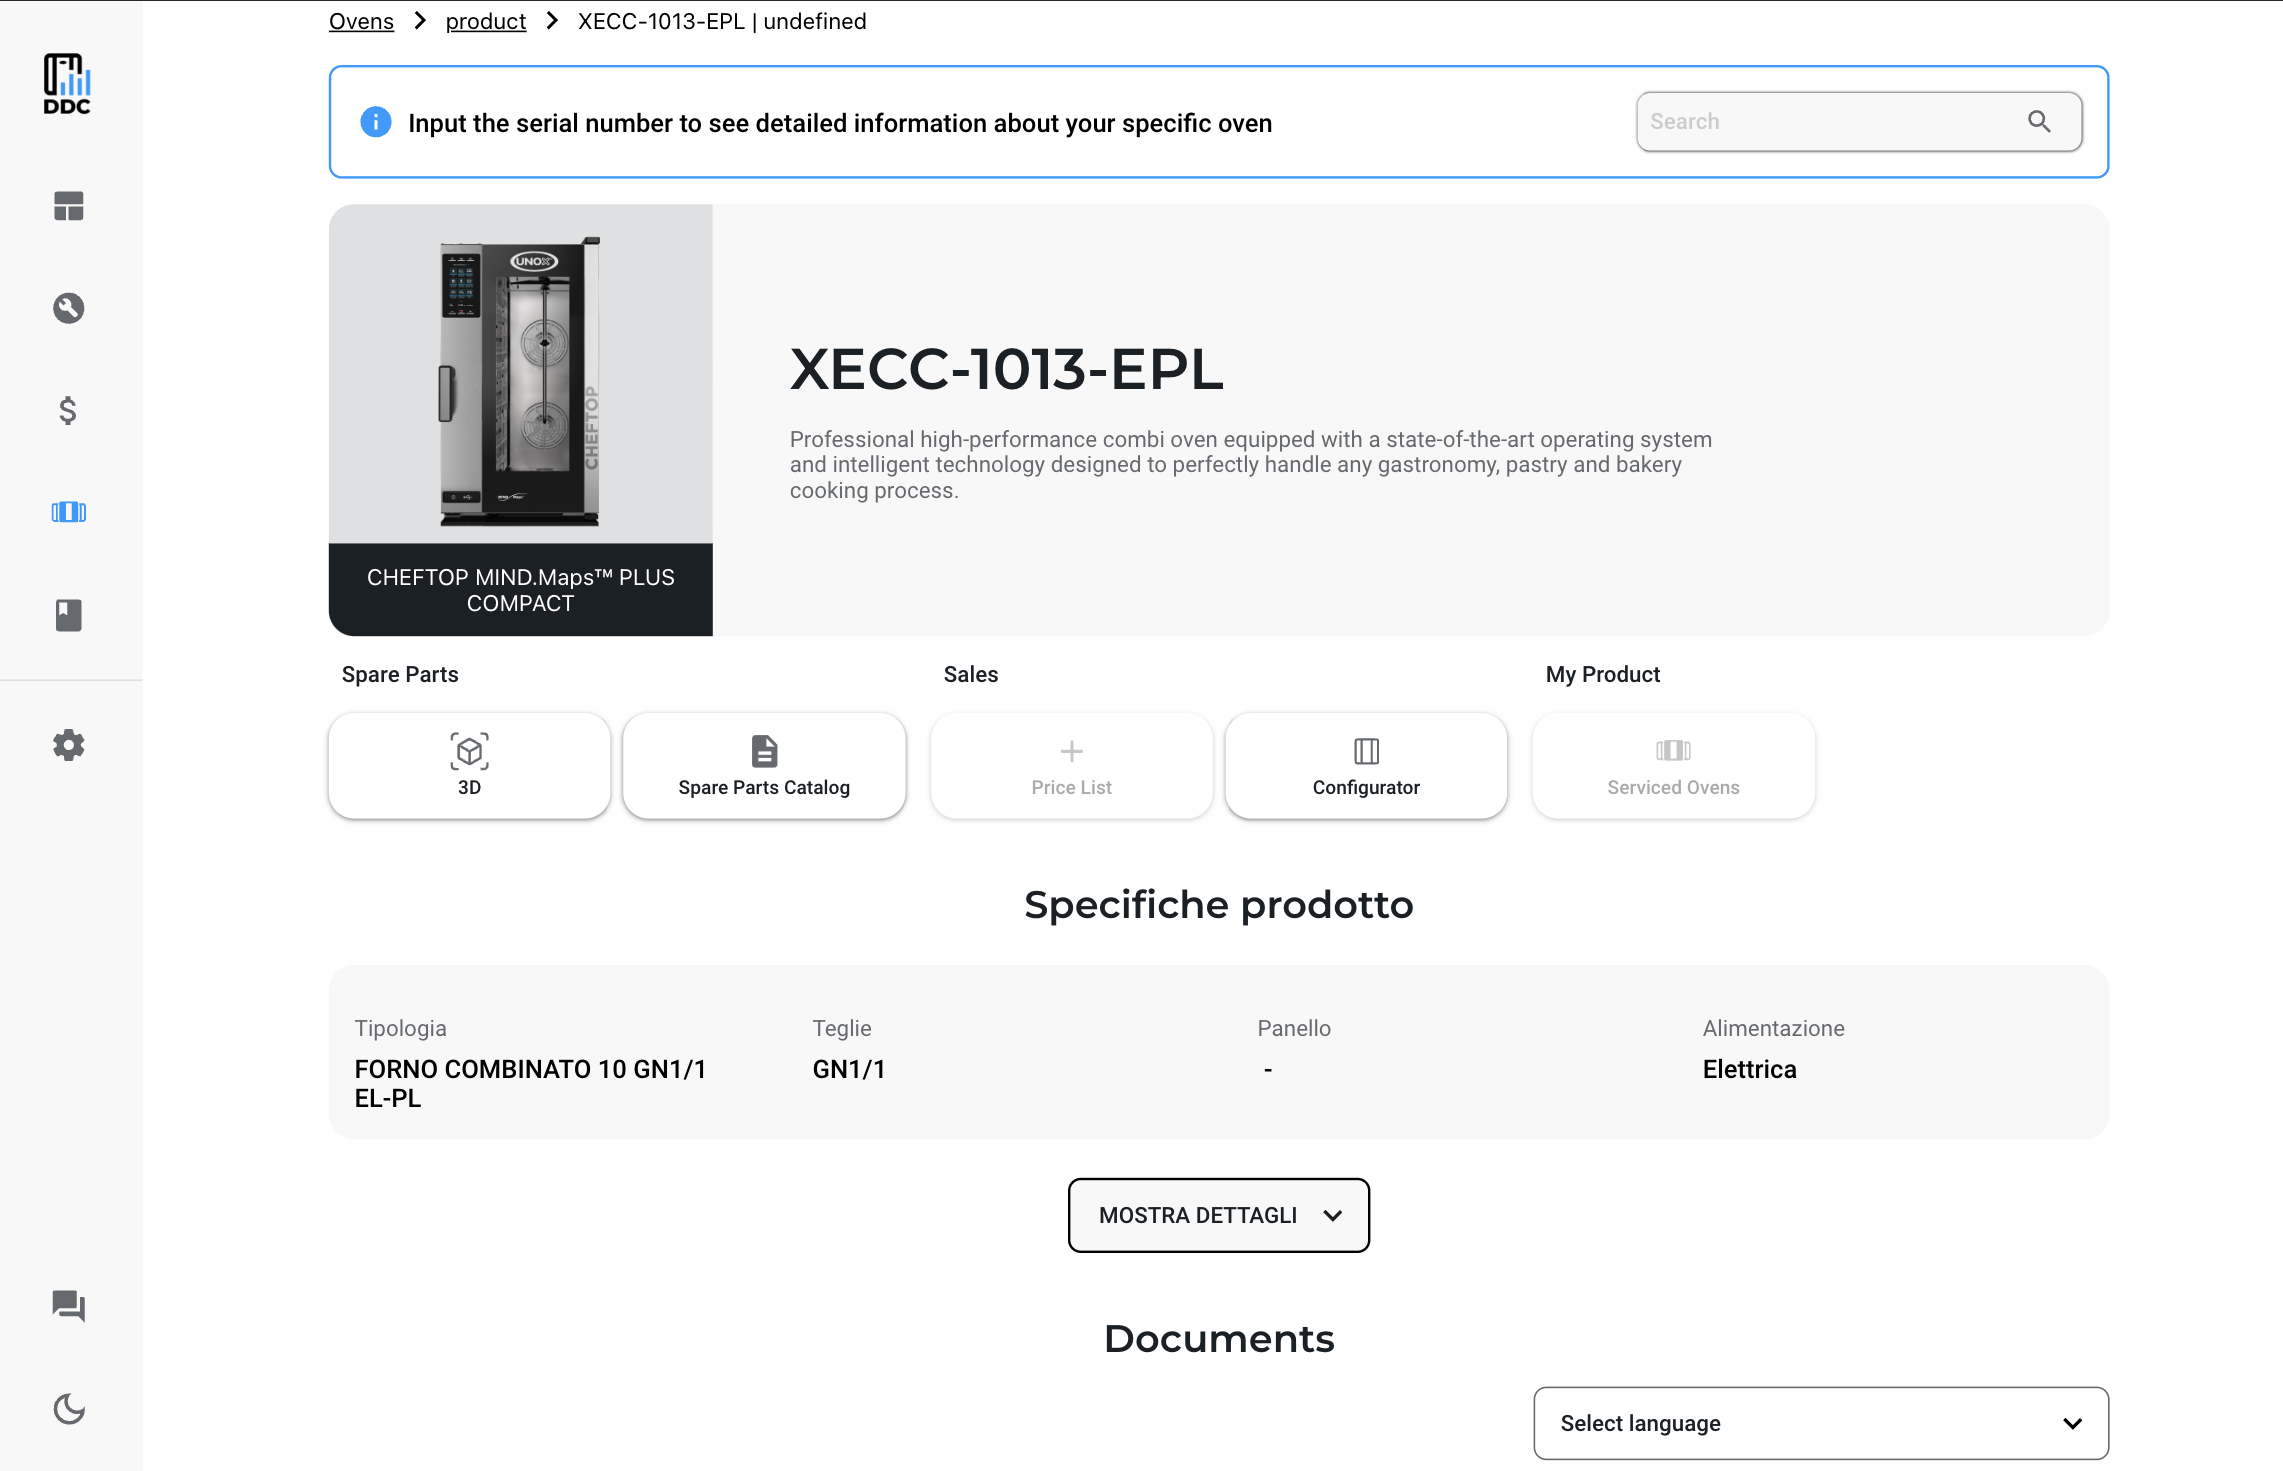
\includegraphics[alt={Screenshot della pagina \textit{"Product Page"} su piattaforma \textit{web}}, height=10cm]{img/ProductPageWeb}
    \caption{App \textit{DDC Service} pagina \textit{Product Page} piattaforma \textit{Web}}
    \label{fig:productpageweb}
\end{figure}

La figura mostra la pagina \textit{"Product Page"} della piattaforma \textit{web} dell'applicazione \textit{DDC Service}.

\begin{figure}[H]
    \centering
    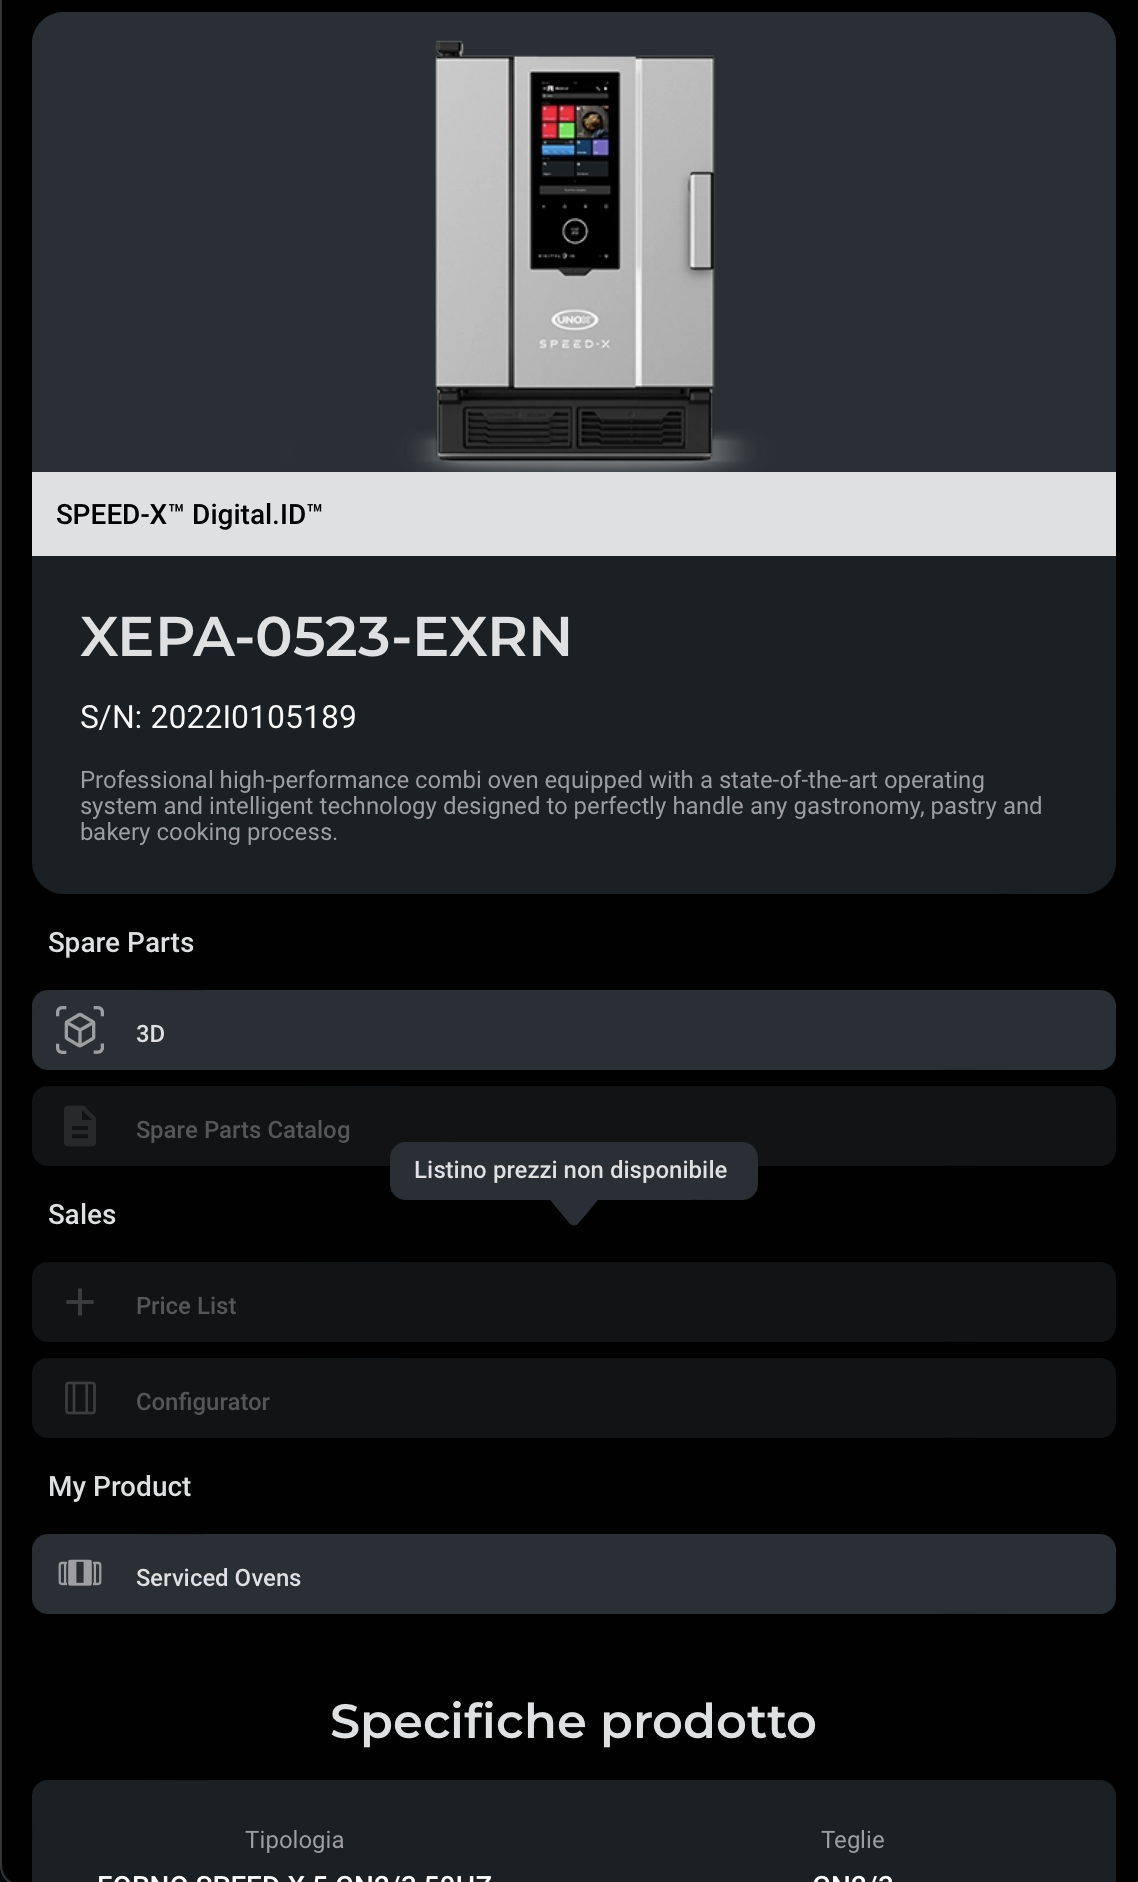
\includegraphics[alt={Screenshot della pagina \textit{"Product Page"} su piattaforma \textit{mobile}}, height=15cm]{img/ProductPageMobile}
    \caption{App \textit{DDC Service} pagina \textit{Product Page} piattaforma \textit{Mobile}}
    \label{fig:productpagemobile}
\end{figure}

La figura presenta la stessa pagina \textit{"Product Page"}, ma su piattaforma \textit{mobile}.
L'applicazione è stata ottimizzata per garantire un'esperienza d'uso eccellente anche su dispositivi \textit{mobile}, con un \textit{design} responsivo che si adatta a diverse dimensioni di schermo.

\begin{figure}[H]
    \centering
    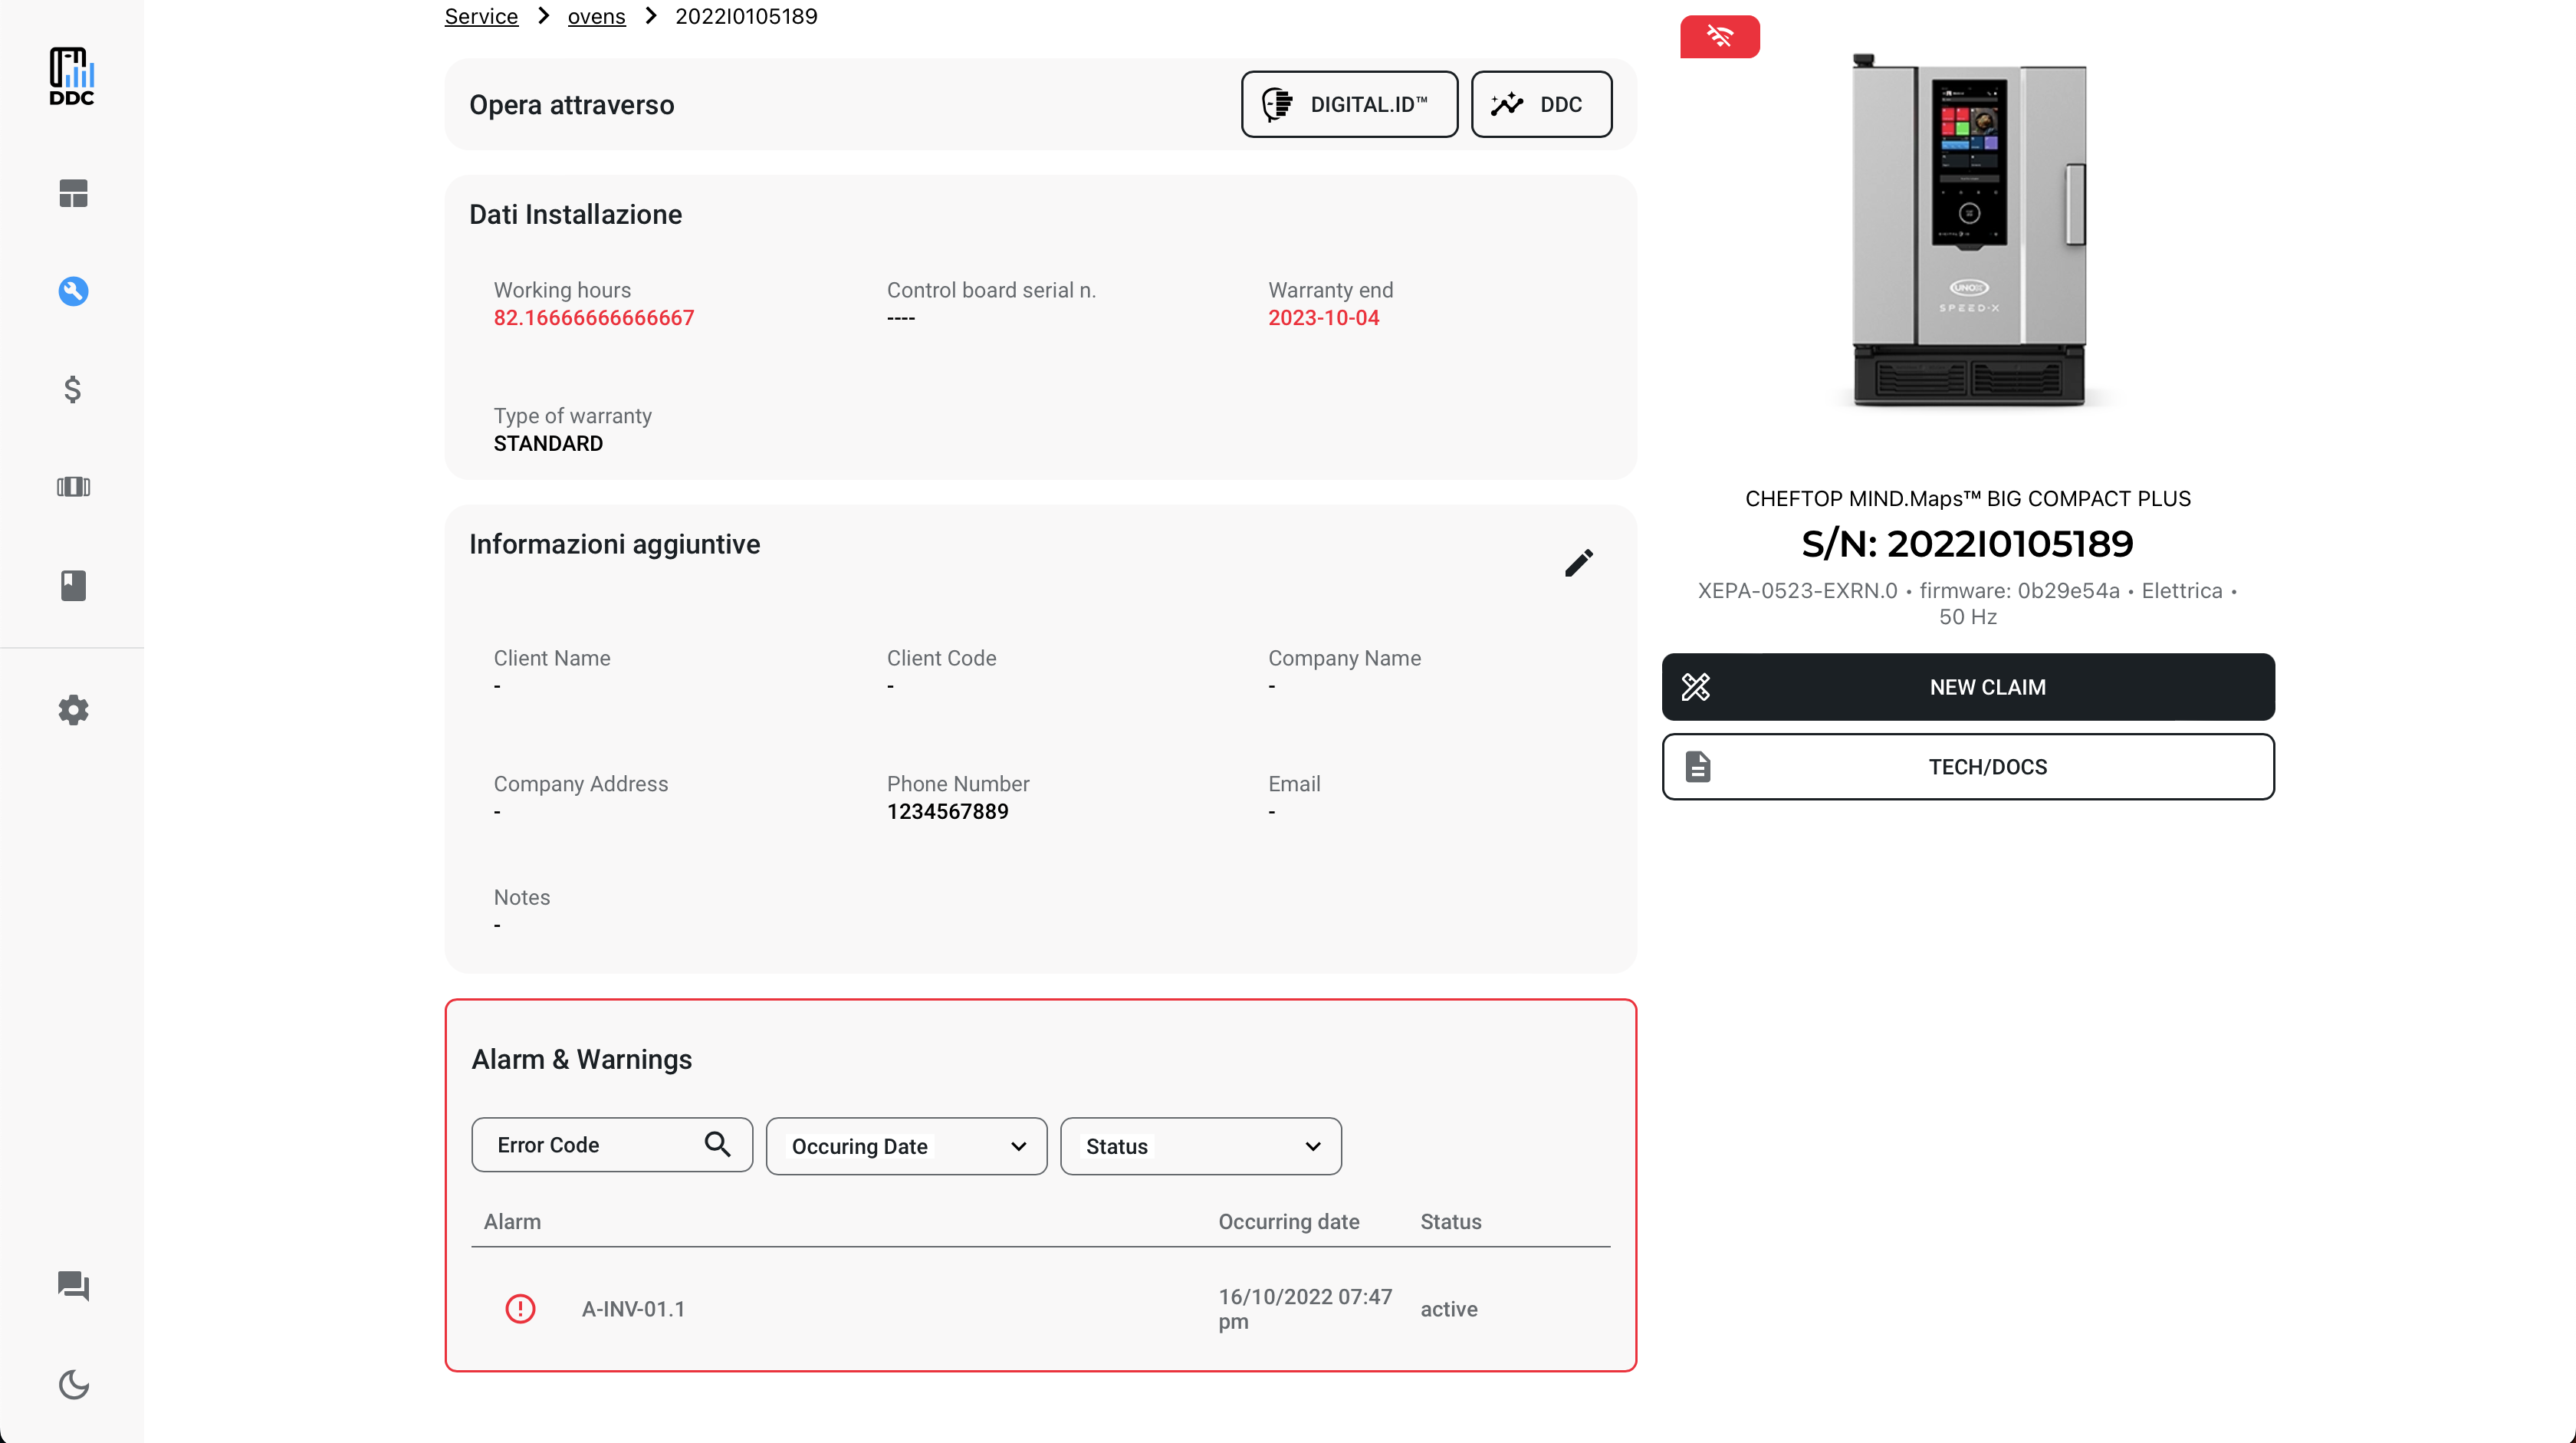
\includegraphics[alt={Screenshot della pagina \textit{"Serviced Oven"} su piattaforma \textit{Web}}, height=10cm]{img/ServicedOvenWeb}
    \caption{App \textit{DDC Service} pagina \textit{Serviced Oven} piattaforma \textit{Web}}
    \label{fig:servicedovenweb}
\end{figure}

La figura \ref{fig:servicedovenweb} illustra la pagina \textit{"Serviced Oven"} sulla piattaforma \textit{Web} dell'applicazione.
Questa pagina permette agli utenti di gestire i forni che necessitano di assistenza.
\section{Conoscenze acquisite}

Durante il mio \textit{stage}, ho avuto l'opportunità di acquisire una vasta gamma di conoscenze e competenze, sia tecniche che organizzative. È stato il mio primo impiego \textit{full-time}, che mi ha dato l'opportunità di acquisire conoscenze sul mondo del lavoro, sulla struttura organizzativa di un'azienda, e sulle attività svolte al suo interno.

\subsection{Competenze Organizzative}

Tra le \textit{soft skill} che sono riuscito a sviluppare durante questo periodo di stage posso enumerare:
\begin{itemize}
    \item \textbf{Gestione del tempo e pianificazione delle attività}: Ho imparato a gestire il mio tempo in modo efficiente e a pianificare le attività per rispettare le scadenze.
    \item \textbf{Collaborazione tra team}: Ho migliorato le mie capacità di comunicazione e di lavoro di squadra, imparando a coordinarmi il lavoro e risolvere i conflitti in modo efficace.
\end{itemize}

È innegabile, però, che molte di più sono state le conoscenze tecniche acquisite in questo periodo.
Di seguito, riporto i principali punti di apprendimento:

\subsection{Gestione delle \textit{Monorepo}}

Uno degli aspetti più significativi del mio lavoro è stato l'apprendimento della gestione delle \gls{monorepog}\glox.
Al giorno d'oggi, l'evoluzione tecnologica è in continua espansione e quello che oggi può essere considerato utile, un domani potrebbe essere considerato \textit{deprecato}.
 Qualsiasi sia il linguaggio di programmazione o il \textit{framework} utilizzato, si parte sempre da un \textit{boilerplate} nei nostri progetti, non capendo realmente cosa quel codice sia o implicitamente imponga.
 Studiare e sapere come funziona una \textit{monorepo} permette di avere gli strumenti per comprendere i progetti e saperli amministrare.
 Nell'ambito dello sviluppo in \textit{Javascript} e in generale con \textit{Node.js}, sapere come gestire le dipendenze in una \textit{monorepo} è una cosa molto importante e questa conoscenza è tra le più importanti che reputo di aver appreso.

Di seguito posso elencare le conoscenze acquisite che reputo più importanti:

\begin{itemize}
    \item \textbf{Centralizzazione delle dipendenze}: Ho appreso i benefici di una centralizzazione delle dipendenze, i vincoli e le sicurezze che garantisce. Questo è particolarmente utile per evitare conflitti e garantire la coerenza tra i vari progetti, oltre che una gestione del \gls{cicdg}\glox migliore.
    \item \textbf{Strumenti di automazione}: Ho imparato a utilizzare strumenti come \textit{Nx}, che facilitano la gestione delle \textit{monorepo} automatizzando compiti comuni come la gestione delle versioni, le pubblicazioni e la condivisione di codice tra i progetti.
\end{itemize}

\subsection{Tecnologie Principali Apprese}

Durante lo stage, ho avuto l'opportunità di lavorare con una serie di tecnologie moderne, migliorando notevolmente le mie competenze tecniche.
La più importante tra tutte è \textit{React} e \textit{React Native} e, in generale, le tecnologie legate allo sviluppo di applicazioni.
Ho imparato a sviluppare utilizzando questa tecnologia, andando nel dettaglio del loro funzionamento e cercando di capire come funzionassero oltre ad utilizzarle e basta.

\begin{itemize}
    \item \textbf{React Native}: Ho approfondito l'uso di \textit{React Native} per lo sviluppo di applicazioni mobili multipiattaforma.
    Ho imparato a creare componenti riutilizzabili, gestire lo stato dell'applicazione con \textit{Redux} e utilizzare \textit{framework} come \textit{Expo}.
    Questa tecnologia mi ha permesso di sviluppare applicazioni efficienti e di alta qualità per diverse piattaforme con una base di codice unica.
    \item \textbf{GraphQL}: Ho acquisito competenze nell'uso di \textit{GraphQL}. Ho imparato i benefici nell'utilizzare questo protocollo di comunicazione nelle \textit{API}.
    \item \textbf{Dripsy/Solito/Moti}: Ho scoperto e utilizzato lo \textit{stack} \textit{Dripsy/Solito/Moti} per la realizzazione di applicazioni multipiattaforma.
    Questo \textit{stack} si è rivelato estremamente utile per gestire con facilità il \textit{routing}, le animazioni e lo stile delle applicazioni.
    \textit{Dripsy} offre una potente libreria per la gestione dello stile in \textit{React Native}, \textit{Solito} facilita il \textit{routing} tra diverse piattaforme e \textit{Moti} semplifica la creazione di animazioni complesse.
\end{itemize}

In sintesi, il mio \textit{stage} è stato estremamente arricchente, permettendomi di acquisire competenze tecniche avanzate e di migliorare le mie capacità organizzative e collaborative.
Queste conoscenze non solo hanno contribuito al successo del progetto di \textit{stage}, ma rappresentano anche un bagaglio prezioso per la mia futura carriera professionale.


\section{Valutazione personale}

Durante il mio percorso di stage, ho avuto modo di mettere in pratica le conoscenze acquisite durante gli studi universitari.
Queste conoscenze mi hanno fornito un solido bagaglio culturale, permettendomi di comprendere e affrontare le sfide del progetto.
Tuttavia, il percorso non è stato privo di difficoltà. Le complessità tecniche e le nuove tecnologie che ho dovuto apprendere hanno reso il lavoro impegnativo, ma estremamente formativo.
I momenti di difficoltà sono stati numerosi, ma proprio grazie a questi ho sviluppato una maggiore persistenza nella risoluzione dei problemi.
Ogni ostacolo superato ha rappresentato un'opportunità di crescita, insegnandomi a non arrendermi di fronte alle sfide e a cercare sempre soluzioni innovative.
L'aspetto più positivo di questa esperienza è stato senza dubbio l'ambiente di lavoro. Ho avuto la fortuna di lavorare in un contesto sereno, dove il rispetto, la collaborazione e il supporto reciproco sono stati fondamentali.
In ogni momento di bisogno, ho potuto contare sull'aiuto di colleghi esperti, che mi hanno guidato e consigliato con professionalità e pazienza.
Il clima lavorativo positivo ha avuto un impatto significativo sulla mia motivazione. Sapere di poter affrontare ogni giornata con serenità mi ha spinto a impegnarmi sempre di più nel progetto, a confrontarmi con i miei colleghi e a continuare a studiare e approfondire le nuove tecnologie.
Questo ambiente mi ha permesso di crescere non solo come professionista, ma anche come individuo, sviluppando una maggiore fiducia nelle mie capacità.
Dal punto di vista educativo, questo stage è stato estremamente prezioso. Ho avuto l'opportunità di lavorare con tecnologie moderne e rilevanti nel mondo del lavoro, ampliando notevolmente il mio bagaglio culturale.
Queste competenze tecniche saranno sicuramente un valore aggiunto per la mia carriera futura, permettendomi di affrontare con maggiore sicurezza e competenza i progetti che verranno.
L'aspetto più importante che questo stage mi ha trasmesso è una nuova capacità di esaminare i problemi e un approccio più pragmatico nell'apprendimento.
Ho imparato a valutare le situazioni in modo critico, a identificare le soluzioni più efficaci e a implementarle.

\pagebreak
In conclusione, posso dire che questa esperienza di stage è stata estremamente positiva. Mi ha permesso di crescere professionalmente e personalmente, offrendomi un'opportunità unica di apprendimento e sviluppo. Sono grato per il supporto ricevuto e per l'ambiente di lavoro stimolante, che mi ha permesso di affrontare con successo le sfide e di acquisire competenze che mi accompagneranno per tutta la vita.


\newpage